\documentclass[12pt]{fphw}

\usepackage[utf8]{inputenc} % Required for inputting international characters
\usepackage[T1]{fontenc} % Output font encoding for international characters
\usepackage{mathpazo} % Use the Palatino font
\usepackage{graphicx} % Required for including images
\usepackage{booktabs} % Required for better horizontal rules in tables
\usepackage{amsmath}
\usepackage{hyperref}

\usepackage{xcolor}

\definecolor{codegreen}{rgb}{0,0.6,0}
\definecolor{codepurple}{rgb}{0.58,0,0.82}

\usepackage{listings} % for importing & highlighting code
\lstdefinestyle{mystyle}{
  commentstyle=\color{codegreen},
  keywordstyle=\color{blue},
  numberstyle=\tiny\color{codegray},
  stringstyle=\color{codepurple},  
  basicstyle=\ttfamily\footnotesize,
}
\lstset{style=mystyle}

\setlength{\parindent}{0in}

%----------------------------------------------------------------------
%	ASSIGNMENT INFORMATION
%----------------------------------------------------------------------

\title{Project}
\author{Aljaž Mur Eržen, Jakob Gaberc Artenjak}
\date{\today}
\institute{Faculty of computer and information science \\ Univerisity of Ljubljana}
\class{Big data}

%----------------------------------------------------------------------

\begin{document}

\maketitle

\section{Problem}

New York City Open Data is a website that contains many different datasets that are produced or in use by the city of New York, USA. One of the datasets, titled "Parking Violations Issued" \cite{violations-2021} contains information about 15M fines issued for parking violations for each of the years from 2014 onwards.

Our task was to handle the dataset, explore its contents and apply basics of machine learning, all while using big data approaches.

\section{Task 1: data formats}

To get started, we converted the dataset from its original CSV format to a few different formats and applied a few different compression algorithms to see, which format is the most suitable for use further on.

\begin{table}[h!]
\begin{center}
\begin{tabular}{l l r}
  Format & Compression & Size \\
  \hline
  parquet        & gzip                & 339 MB \\
  parquet        & brotli              & 398 MB \\
  avro           & snappy              & 662 MB \\
  parquet        &                     & 671 MB \\
  avro           &                     & 2.2 GB \\  
  HDF            & zlib, comp. level=9 & 2.2 GB \\
  CSV (original) &                     & 2.2 GB \\
  HDF            &                     & 2.6 GB \\
\end{tabular}
\caption{Comparison of sizes produced by different storage formats}
\label{table-formats}
\end{center}
\end{table}

One can see that HDF is not efficient at all. Without compression, the size of the dataset actaully grew when converted from plain-text CSV. 

Most efficient format was parquet with gzip compression, which produced not only the smallest output, but has also been comparable to other formats in terms of time required for the compression.

Parquet is a file format developed by Apache Fundation. It stores tabular data, organized in rows and columns, but contrary to CSV and most relational databases, it does not store data by rows, but by columns. This approach is called columnar storage and is beneficial because of the fact that usually, values in the same column are more similar than values in the same row, which may differ even in their data type. 

\section{Task 2: augemtation}

\section{Task 3: exploration}

\begin{figure}[h!]
  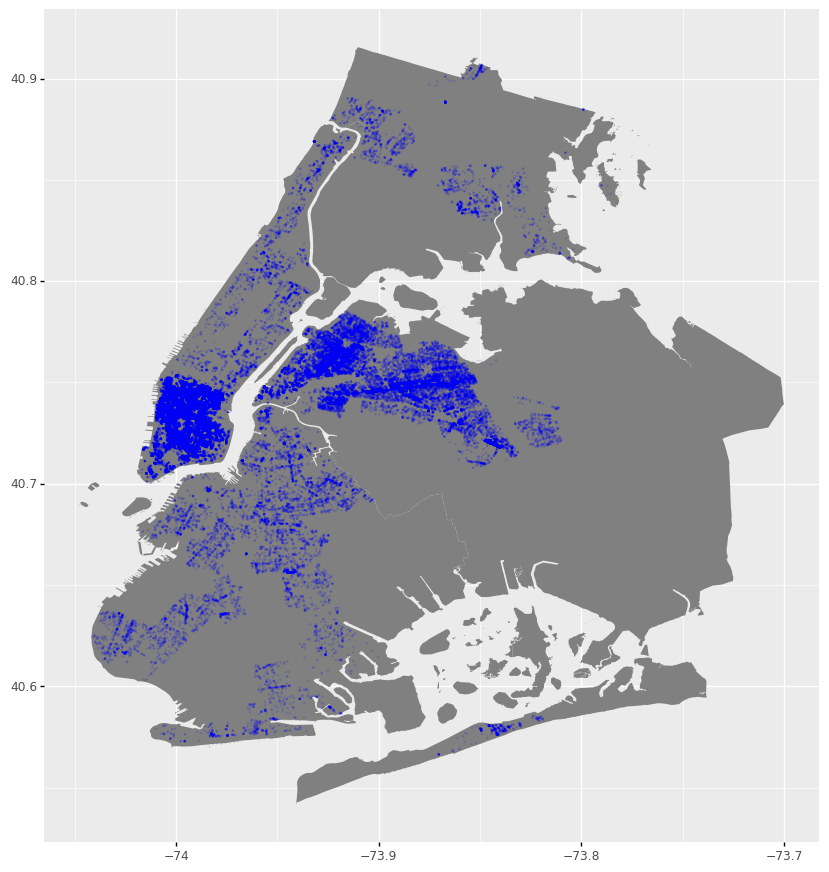
\includegraphics[width=1\textwidth]{figures/nyc.map.png}
  \caption{Locations of violations in the year 2022 in the months January to May}
\end{figure}




\begin{thebibliography}{9}

\bibitem{violations-2021}
  City of New York, Open Data,
  \href{https://data.cityofnewyork.us/City-Government/Parking-Violations-Issued-Fiscal-Year-2021/kvfd-bves}{\emph{Parking Violations Issued - Fiscal Year 2021}},

\bibitem{jq}
  jq,
  \href{https://stedolan.github.io/jq/}{\emph{Lightweight and flexible command-line JSON processor}},

\bibitem{json-path}
  \href{https://goessner.net/articles/JsonPath/}{\emph{JSON path}},

\bibitem{graphql}
  GraphQL,
  \href{https://graphql.org/}{\emph{A query language for your API}},

\bibitem{partiql}
  PartiQL,
  \href{https://partiql.org/}{\emph{SQL-compatible access to relational, semi-structured, and nested data.}},

\bibitem{json-query}
  \href{https://www.npmjs.com/package/json-query}{\emph{json-query}},


\bibitem{streamz}
  Graham Cormode; Muthu Muthukrishnan,
  \href{https://ieeexplore.ieee.org/document/6042851}{\emph{Approximating Data with the Count-Min Sketch}}.


\end{thebibliography}

\end{document}